\documentclass[a4paper,10pt,journal]{IEEEtran}

% Extension packages providing additional functionality
\usepackage{amsmath}       % additional math environments
\usepackage{graphicx}      % graphics import from external files
\usepackage{epstopdf}      % automates .eps to .pdf conversion
% epstopdf package may require --shell-escape option to pdflatex
\usepackage{booktabs}      % table typesetting additions
\usepackage{siunitx}       % number and units formatting
%\usepackage{caption}       % customisation of captions
\usepackage{url}           % format url addresses
%\usepackage{tikz,pgfplots} % diagrams and data plots
 \usepackage{acronym}	%consistent acronym handling

% some handy commands for referencing;
% the optional argument overrides the default label, e.g.
% \figref[FIG.~]{fig:label}
\newcommand{\figref}[2][\figurename~]{#1\ref{#2}}
\newcommand{\tabref}[2][\tablename~]{#1\ref{#2}}
\newcommand{\secref}[2][Section~]{#1\ref{#2}}

%	\renewcommand{\vec}[1]{\mathbf{#1}}	%bold vectors


\begin{document}

\title{Nanocomposite Design of Thermoelectric Materials\\Introductory
Report}
\author{\IEEEauthorblockN{Callum Vincent}\\
\IEEEauthorblockA{cv235@exeter.ac.uk\\24 November 2013}
}

\IEEEaftertitletext{\vspace{-1\baselineskip}\noindent
%\begin{abstract}
Thermoelectrics are a promising area of materials research recently
revitalised by the introduction of nanocomposites. Obtaining a
thermoelectric figure of merit $ZT > 3$, potent new energy applications
are attainable. Current bulk thermoelectric materials reach $ZT < 1$,
realising practical efficiencies of ~4\%.\\
Reductions of # in phonon thermal conductivity $kappa_{ph}$ have been
suggested \cite{crc-handbook}, with potential for $ZT > #$. Applying the
Boltzmann transport equation to the phonon and \acronym{NFE}{nearly
free electron} models for the concept of \acronym{PGEC}{phonon glass
electron crystal} \cite{crc-handbook}, we search for a theoretical
mechanism through which $kappa_{ph}$ can be reduced. If such a
mechanism is discovered, we will design and computationally model new
material structures to demonstrate its validity.
\end{abstract}

\vspace{1\baselineskip}}

\maketitle

\section{Introduction}

From its discovery in 1821, thermoelectricity has seen constant
attention by the scientific community. Its source lies deep in the
fundamental nature of solid state materials. Through understanding
thermoelectricity we meld all the concepts underpinning
\acronym{SSP}{solid-state physics}; a well defined thermoelectric
theory is the pinnacle of \ac{SSP}.

%citations below? for the numbers?

Thermoelectricity is not only a central area of research for
\ac{SSP}, but also has enormous practical significance. Current
bulk thermoelectrics achieve thermoelectric figure of merit $ZT$ up to
one, which results in a practical thermal efficiency (heat to work) of
just 4\%, six times less than modern internal combustion engines.\\
Despite this low figure, thermoelectrics still see niche use
in refrigeration and space exploration due primarily to their
exceptional reliability. By increasing $ZT$ up to three, new
applications in heat recovery systems and solar thermal generators
emerge, improving the thermal efficiency of current power generation
methods. Theoretically, there is no upper limit to $ZT$, and as it
approaches infinity, efficiencies at the Carnot limit can be obtained.
If we achieve $ZT \to\infty$, all heat gradients will be maximally
exploitable for high value electrical energy; once where there were
water wheels, there became hydroelectric dams, now where there is
heat, there will be thermoelectricity.

% Change the section name?
\section{Background Theory}
\subsection{Thermoelectricity}
In 1821, Thomas Seebeck discovered that a circuit made from two
dissimilar metals, with junctions at different temperatures would
deflect a compass magnet (\figref{seebeck-experiment}), he had
discovered thermoelectricity. The temperature gradient $\vec{\nabla}
T$ between the junctions generates an electromotive force:

\begin{equation}
\label{seebeck-emf}
	\vec{E_{emf}} = -S \vec{\nabla} T
\end{equation}
where $S$ is the Seebeck coefficient, defined as the induced voltage per
unit temperature difference, mathematically $\Delta S = \frac{\Delta
V}{\Delta T}$ \cite{auparay}. This coefficient is not only material
dependent, but also temperature dependent, i.e., a temperature gradient
produces an electromotive force gradient. This electromotive force
gradient produces a current density gradient described macroscopically
by a modified Ohm's law \cite{ziman}:

\begin{equation}
\label{current-density}
	\vec{J} = \sigma (-\vec{\nabla} V - S \vec{\nabla} T)
\end{equation}
where $\vec{J}$ and $\sigma$ are the current density $\frac{I}{A}$ and
electrical conductivity at a given location in the material and
$\vec{\nabla} T$ and $\vec{\nabla} V$ are the temperature and
resultant voltage gradients across the material. If we were to repeat the
experiment conducted by Seebeck (\figref{seebeck-experiment}), using a
probe to measure $V$ between junctions and $\sigma$ at each junction
for one of the metals, assuming steady state, i.e., $I=0 \therefore
\vec{J} = 0$, the metals Seebeck coefficient can be determined.\\
Thermoelectricity, its uses and current nanocomposite research are well
summarised by J. W. Bos \cite{bos-review} and A. J. Minnich et al.
\cite{minnich-review}.

\begin{figure}
	\centering
	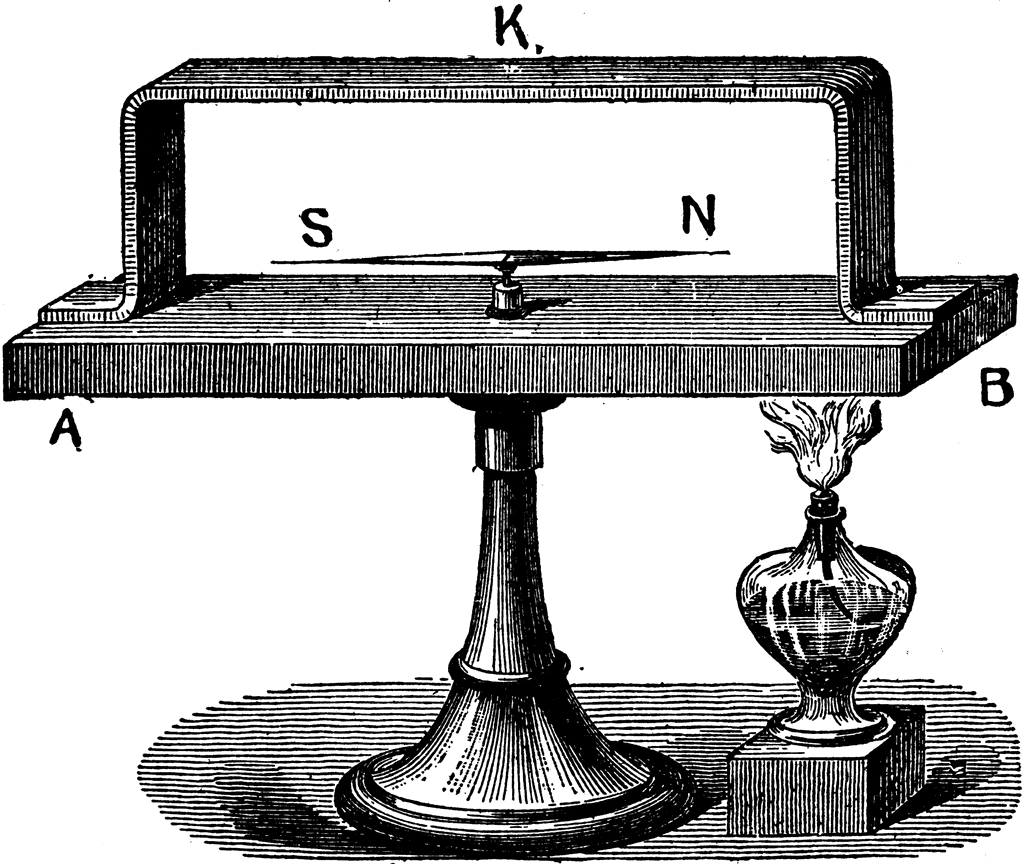
\includegraphics[width=0.5\textwidth]{seebeck-experiment-black.png}
	\caption{Thomas Seebeck's original thermoelectricity experiment
	diagram \cite{seebeck-original}. A compass needle lies on top of
	one metal, underneath a bridge of a different metal (K), connected
	by two junctions and heated at one of these junctions.}
	\label{seebeck-experiment}
\end{figure}

\subsection{Statistical Mechanics}
Using the kinetic theory, with relevant assumptions, charge density
$\vec{J}$ of an arbitrary charge carrier can be described
microscopically \cite{kittel}:

\begin{equation}
\label{charge-density}
	\vec{J} = \frac{nq^2\vec{E} \tau}{m}
\end{equation}
where $n$ is free charge carrier density, $q$ is the charge of the
carrier, $\vec{E}$ is the electric field accelerating the
carrier, $\tau$ is the mean time between carrier collisions and $m$ is
carrier mass.\\
Applying this to solid-state electrical conductivity $\sigma = \frac{ne^2
\tau}{m^*}$ it can be shown that \cite{ziman}:

\begin{equation}
\label{micro-elec}
	\sigma = \frac{e^2}{m^*} \sum_{\mathrm{spin}} \sum_{\vec{k}}
	n(\vec{k}) \tau(\vec{k})
\end{equation}
where $m^*$ is the electron effective mass, $\mathrm{spin}$ refers to
electron spin and $\vec{k}$ is the electron wavevector over the
Brillouin zone. These new concepts are all derived from the \ac{NFE}
model, as described in Kittel \cite{kittel}.\\
The Boltzmann transport equation "describes the statistical behaviour
of a thermodynamic system not in thermodynamic equilibrium"
\cite{wiki-boltz} and its general definition is:

\begin{equation}
\label{boltz-trans}
	\frac{\partial f}{\partial t} = \left(\frac{\partial f}{\partial
	t}\right)_\mathrm{force} + \left(\frac{\partial f}{\partial t}\right)_\mathrm{diff}+ \left(\frac{\partial f}{\partial t}\right)_\mathrm{coll}
\end{equation}
where $\frac{\partial f}{\partial t}$ is time dependence of a system
of particles $f$, the "force" term represents external forces on the
particles, the "diff" term is the diffusion of particles through the
system and the "coll" term represents forces acting between particles
in collisions.\\
A phonon is the quantisation of vibrational motion of a lattice of
atoms at a single frequency, known as a normal mode. These phonons are
quasiparticles, free to move around the lattice and they are
distributed according to the Bose-Einstein distribution \cite{kittel}:

\begin{equation}
\label{bose-einstein}
	 \bar{n} = \frac{1}{e^{(\hbar \omega) / k T} - 1}
\end{equation}
where $\bar{n}$ is the probability of a phonon existing with energy
$\hbar \omega$.\\
Electrons can be modelled as quasiparticles in a similar way, with a
wavevector and effective mass as in equation \eqref{micro-elec},
leading to the Fermi-Dirac distribution \cite{kittel}:

\begin{equation}
\label{fermi-dirac}
	 \bar{f} = \frac{1}{e^{(E - E_f) / k T} + 1}
\end{equation}
where $\bar{f}$ is the probability of an electron existing with energy
$E$ and $E_f$ is the Fermi level.\\
In the presence of an external fields, phonon and electron
distributions (\eqref{bose-einstein} \& \eqref{fermi-dirac}) both
satisfy the Boltzmann transport equation \eqref{boltz-trans} with
\cite{ziman}:

\begin{equation}
\label{boltz-specific}
	\frac{df}{dt}\bigg|_{field} + \frac{df}{dt}\bigg|_{collisions} = 0
\end{equation}
where function $f$ is $f = \bar{n}$ or $f = \bar{f}$, the Bose-Einstein
and Fermi-Dirac distribution functions.

\subsection{Nanocomposites}

Composite materials "are materials made from two or more constituent
materials with significantly different physical or chemical
properties, that when combined, produce a material with
characteristics different from the individual
components" \cite{wiki-composite}. Nanocomposites are identical in
concept to traditional composites, except the constituent materials
are at that nanoscale. As our nanocomposites are at a comparable size
to the crystal lattices of their constituent materials, we can view
nanocomposites as artificial defects in a larger crystal lattice. A
simple example of a 2D nanocomposite, a copper-graphene superlattice,
is pictured in \figref{superlattice}. Examining one layer of the
superlattice, the material in bulk form would be a 3D crystal structure,
but by constraining the layer thickness we have introduced a boundary
defect. The periodic array of these boundary defects forms a new 3D
artificial crystal, which we define as a superlattice, a nanocomposite.

2D -> 1D -> 0D

\begin{figure}
	\centering
	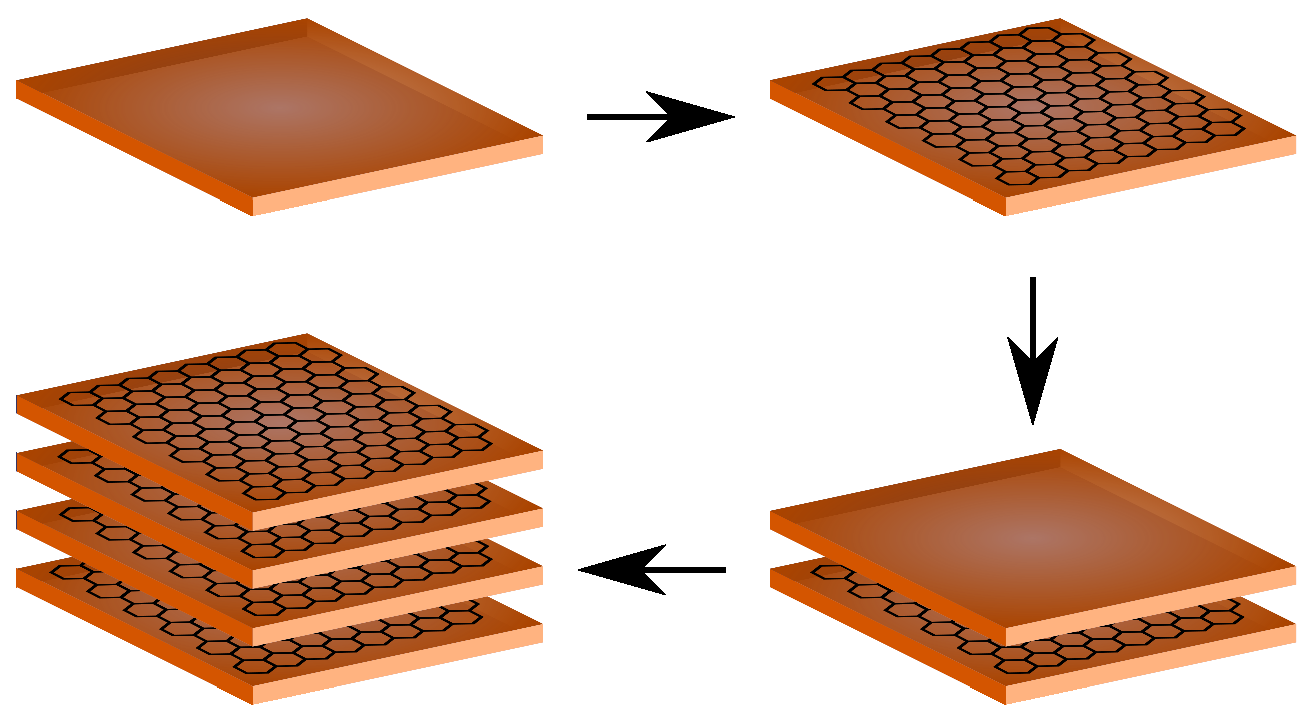
\includegraphics[width=0.5\textwidth]{graphene-superlattice.eps}
	\caption{Superlattice of graphene and copper. Alternate layers of
	nanoscale copper and graphene are sandwiched together.}
\end{figure}

\section{Project Theory Discussion}
\subsection{Assumptions}
For our project we will be using the phonon and \ac{NFE} models, which
bring with them a multitude of assumptions. For the phonon model, our
main assumption is that our system is at least 50 atomic oscillators
\cite{kittel}; this means we are limited to a $50\r{A} = 5
\mathrm{nm}$fabrication size. Current fabrication methods are at best
25nm \cite{minnch-review}, so our 50 oscillator assumption is well met.
For both the phonon and the \ac{NFE} model, we assume an ideal gas,
i.e., particles do not interact with each other and can move freely
around the lattice, effected only by lattice perturbations. This is
known to be a good assumption for the low temperatures in \ac{SSP}
\cite{kittel}.\\
Based on this limited initial analysis, we believe these assumptions
should be valid with an accurate final model possible. If it transpires
that these assumptions cannot be valid, we will seek alternative models.\\

\subsection{Thermoelectric Efficiency}
The thermoelectric efficiency is best expressed in the dimensionless
parameter $ZT$ with thermal efficiency $\eta = \eta (Z\bar{T}, T_h,
T_c)$, where $Z$ is the figure of merit, $\bar{T} = \frac{1}{2}(T_h +
T_c)$, $T_h$ is the temperature at the hot junction and $T_c$ is the
temperature at the cold junction. Note that the $T$ in the commonly
cited $ZT$ really refers to $Z \bar{T}$. This is omitted due to the
temperature appearing of both sides of the expression for $ZT$:
\begin{equation}
\label{zt}
	Z \bar{T} = \frac{S^2 \sigma \bar{T}}{\kappa_e + \kappa_{ph}}
\end{equation}
where $S$ is the Seebeck coefficient from equation \eqref{seebeck-emf}
\& \eqref{current-density}, $\sigma$ is electrical conductivity,
$\kappa_e$ and $\kappa_{ph}$ are the thermal conductivity due to
electrons and phonons. This is derived in D. M. Rowe's Modern
Thermoelectrics \cite{modern-thermoelectrics}.\\
Current thermoelectric materials $ZT$ values against temperature are
plotted in figure \figref{zt-plot}

\begin{figure}
	\centering
	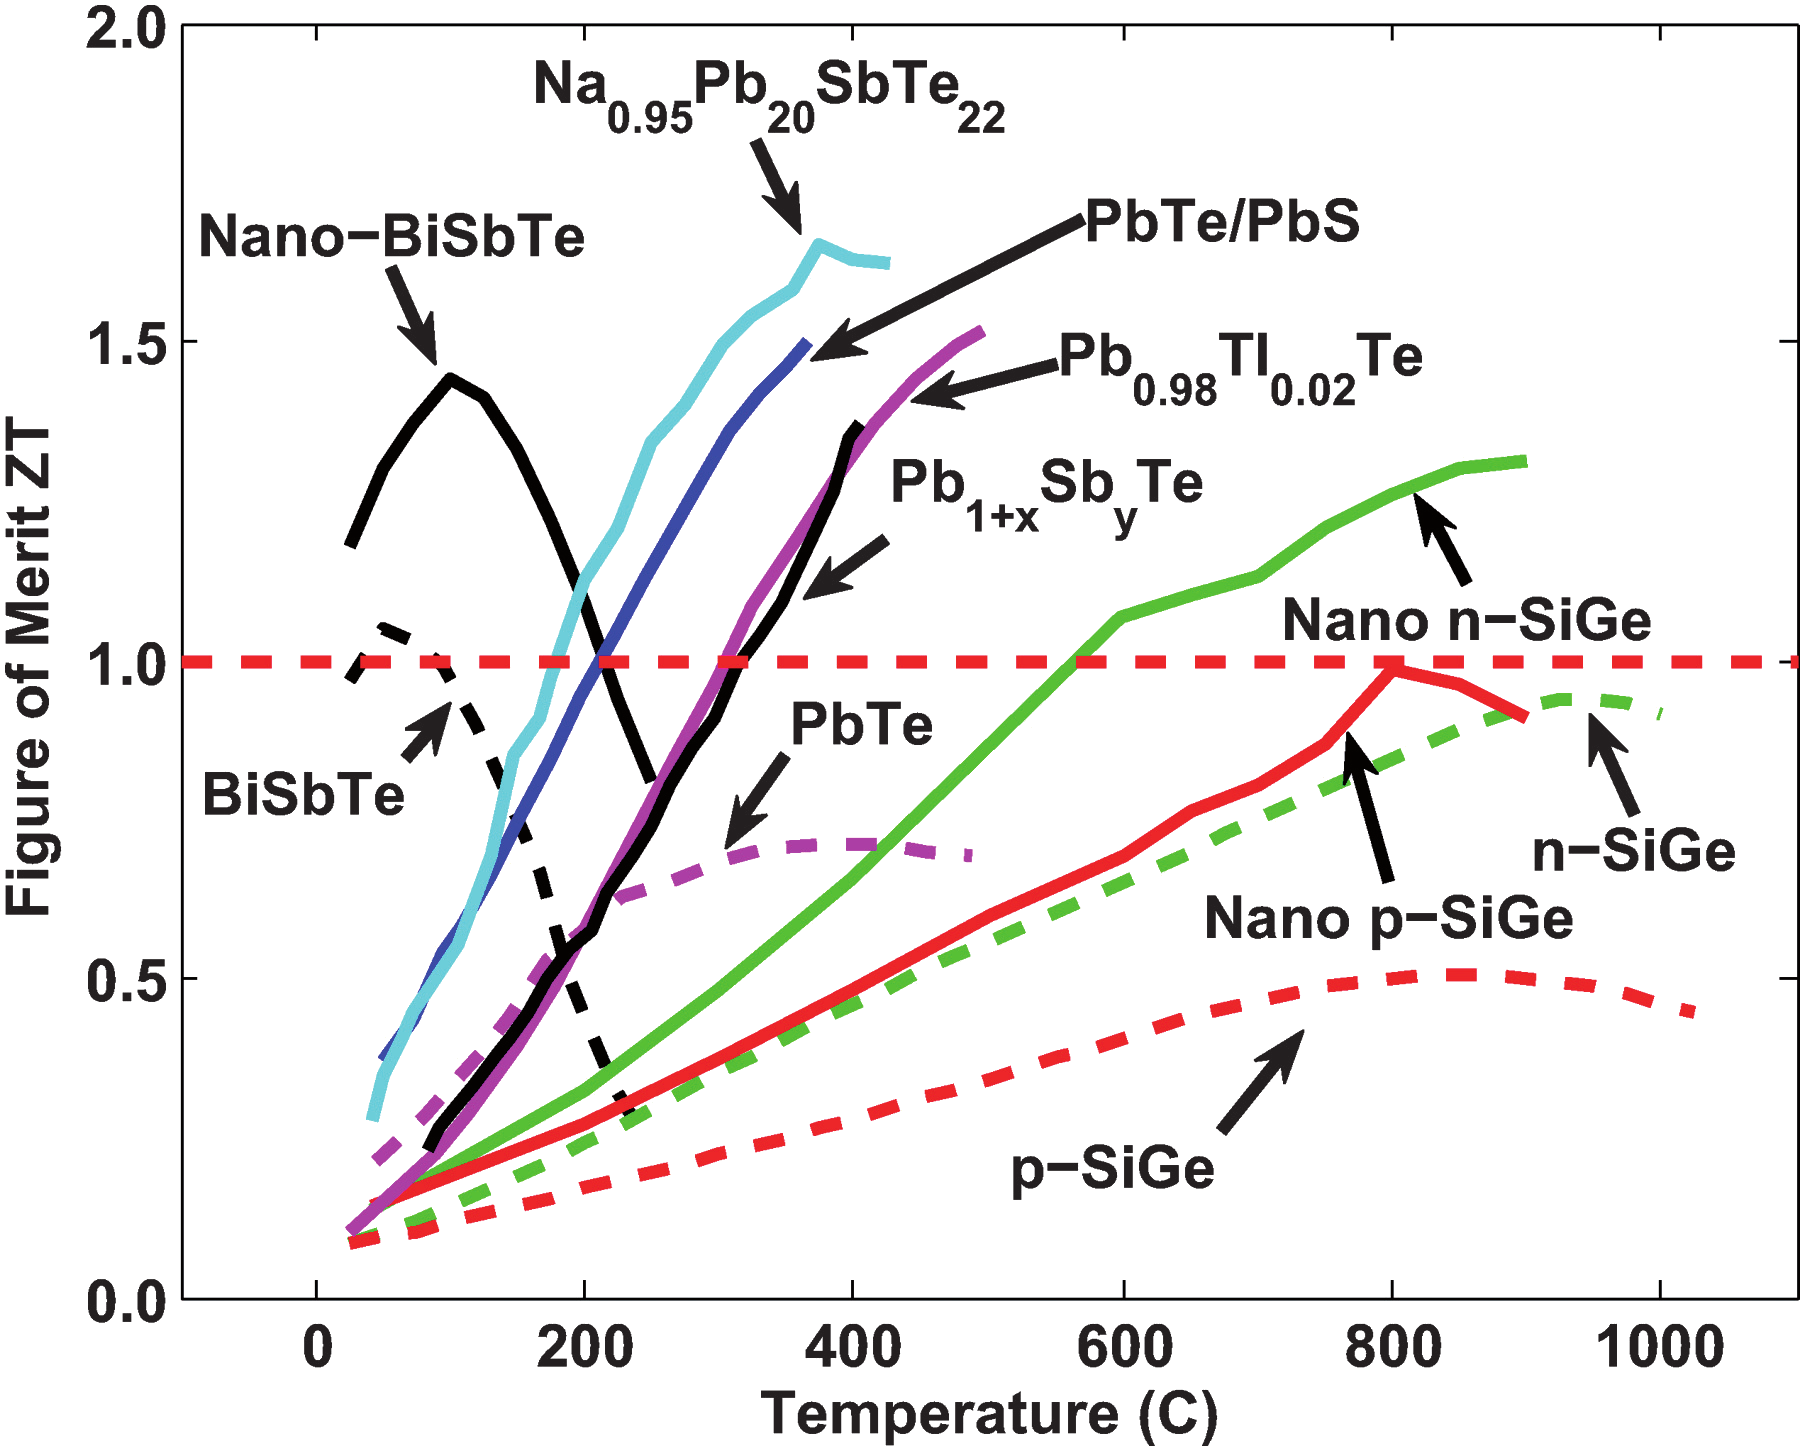
\includegraphics[width=0.5\textwidth]{zt-temp-plot.png}
	\caption{Plot of thermoelectric figure of merit $ZT$ against
	temperature. Note $ZT$ is proportional to the thermal efficiency
	$ZT \propto \eta$ \cite{minnich-review}.}
\end{figure}

The mean time between collisions $\tau$ from \eqref{charge-density} is
of vital importance for our project.

\subsection{\acf{PGEC}}
A core research topic for our project is the idea of \ac{PGEC}. How can
we achieve this? What are the constraints?

\section{Conclusions \& Project Aims}
Thermoelectric theory provides a good basis from which we can
understand \ac{SSP}. Using phonon and \ac{NFE} models together with
the Boltzmann transport equation \eqref{boltz-trans} we aim to develop
a \ac{PGEC} inspired mechanism through which $ZT$ can be improved and
test this mechanism computationally. In pursuit of this aim, it is
likely that we utilise nanocomposite material design for the
introduction of multiple boundary defects.

\bibliographystyle{IEEEtran}
\begin{thebibliography}{2}
\bibitem{crc-handbook}
G. A. Slack, \emph{CRC Handbook of Thermoelectrics}. Ed D. M. Rowe, CRC Press, 1995
\bibitem{seebeck-original}
\url{etc.usf.edu/clipart/35600/35659/seebeck_35659_lg.gif} 24 November
2013
\bibitem{auparay}
N. Auparay, \emph{Room Temperature Seebeck Coefficient Measurement
of Metals and Semiconductors}. Available
from:
\url{http://www.physics.oregonstate.edu/~tate/TateLabWiki/lib/exe/fetch.php?media=theses:auparay_bs_2013.pdf} 20 November 2013
\bibitem{bos-review}
J. W. Bos, \emph{Thermoelectric materials: efficiencies found in
nanocomposites}. Education in Chemistry, March 2012. Available
from:
\url{http://www.rsc.org/images/Thermoelectric-materials_tcm18-214041.pdf} 24 November 2013
\bibitem{minnich-review}
A. J. Minnich et al. \emph{Bulk nanostructured thermoelectric
materials: current research and future prospects}. Energy Environ.
Sci., 2009, 2, 466-479. DOI: 10.1039/B822664B
\bibitem{ziman}
%p270-275, section 7.5 & 7,6
J. M. Ziman, \emph{Electrons and Phonons: The Theory of Transport
Phenomena in Solids}. 1960, ISBN: 978-0-19-850779-6
\bibitem{kittel}
C. Kittel, \emph{Introduction to Solid State Physics, 8th ed}. November 2004, ISBN: 978-0471415268
\bibitem{wiki-boltz}
\url{http://en.wikipedia.org/wiki/Boltzmann_equation} 18 November 2013
\bibitem{wiki-composite}
\url{http://en.wikipedia.org/wiki/Composite_material} 22 November 2013
\bibitem{modern-thermoelectrics}
D. M. Rowe, \emph{Modern Thermoelectrics}. Reston Pub Co, September
1983. ISBN: 978-0835945936
\end{thebibliography}

\end{document}

%shifted out of document probably not going to use
\newpage
\appendix
\section{Acronym List}
\acresetall
\ac{PGEC} - Exhibiting the properties of phonon scattering glasses and
electron transmissive crystals
\ac{SSP} - The study of rigid matter (solids)

\section{Open Questions}
These questions are ideas that I have posed thus far in the project.
They are included as an interest to the reader, perhaps indicating
area of further study

\begin{itemize}
  \item Can acoustic stimulation of a material cause additional phonon
  collisions? Is a $kappa_{ph}$ reduction obtainable?
\end{itemize}